\documentclass{article}
\usepackage[utf8]{inputenc}
\usepackage[spanish]{babel}
\usepackage{listings}
\usepackage{color}
\definecolor{miverde}{rgb}{0,0.6,0}
\usepackage{graphicx}
\graphicspath{ {images/} }
\usepackage{cite}
\usepackage{comment}
\usepackage{subfig}
\usepackage{adjustbox}
\usepackage{float}
\usepackage[colorlinks=true,urlcolor=blue,linkcolor=black,citecolor=blue]{hyperref}
	\urlstyle{same}
\usepackage{cite}

\usepackage{geometry}
\geometry{left=21mm,right=18mm,top=23mm,bottom=23mm,headheight=15pt} 	



\begin{document}

\begin{titlepage}
    \begin{center}
        \vspace*{2cm}
            
        \Huge
        \textbf{`Nada es lo que parece' \\
        Proyecto de encriptación de información}
            
        \vspace{0.5cm}
        \LARGE
        Parcial 1\\
        Informática 2

        
            
        \vspace{2,5cm}
            
        \textbf{
        Katherin Johana Henao Henao\\
        c.c.1036953583\\
        Diego Alejandro Londoño Jiménez\\
        c.c.71377279\\
        }
            
        \vfill
            
        \vspace{2,5cm}
            
        \Large
        Despartamento de Ingeniería Electrónica y Telecomunicaciones\\
        Universidad de Antioquia\\
        Medellín\\
        Febrero de 2022
            
    \end{center}
\end{titlepage}

\tableofcontents
\newpage

%\thispagestyle{empty}
%\listoffigures
%\newpage
%\listoftables
%\newpage
%\pagenumbering{arabic}

\section{Introducción}
\label{intro}
En el presente proyecto se desarrolla un sistema de transmisión de encriptación que permite cifrar los datos transmitidos entre dos puntos. Es un demo de la transmisión y recepción de información entre las oficinas de una sucursal bancaria, los cuales usan infraestructura cableada para tal fin. La información viaja desde un computador de origen que es el generador de la información, hasta un computador destino que es el que se presenta al encargado de tomar decisiones en la bolsa de valores. \\
Para el desarrollo se hizo uso de la plataforma Tinkercard y de diferentes componentes circuitales como el circuito integrado 75HC595 entre otros. Además todo el desarrollo del proyecto se hace con manejo de repositorios


\section{Justificación} 
\label{contenido}
El flujo actual de información en la web transporta datos sensibles como por ejemplo información bancaria; ante las técnicas para acceso indebido a la información impropia es necesario utilizar diferentes técnicas para protección de los datos. Entre ellos está la encriptación que se ha hecho indispensable porque ayuda a proteger y mantener la confidencialidad de la información cuando esta se envía de un lugar a otro. La encriptación es un método de codificación de la data que permite que solo las partes interesadas puedan comprenderla a pesar de que terceros hayan accedido a ella.

\section{Objetivo general} 
\label{contenido}
Desarrollar en equipo un sistema de encriptación y desencriptación de información entre un transmisor y un receptor utilizando la plataforma Tinkercad

\section{Objetivos específicos} 
\label{contenido}
\begin{itemize}
\item Consolidar las habilidades adquiridas en el lenguaje de programación C++
\item Enlazar los diferentes conocimientos adquiridos en el curso de informática ll 
\item Afianzar el trabajo el equipo en el desarrollo de un proyecto

\end{itemize}
\section{Análisis del problema y consideraciones}
Como se está implementando un sistema de transmisión de información se analiza que será necesario tener dos placas de arduino para que una haga las veces de transmisor y la otra haga las veces de receptor.

La  información entra al arduino vía serial, en este punto la información ya se encuentra encriptada. Como se desconoce la longuitud de la trama encriptada se deduce que se deberá hacer uso de memoría dinámica, haciendo uso de datos tipo puntero.\\

Como se debe tener una seña de reloj para que haya sincronismo en el sistema, se pueden definir dos pines digitales de la placa de arduino como puertos de salida y escribir en estos cambios de estado para simular las señales de reloj que el integrado requiere para su operación correctamente. Acá una consideración a tener en cuenta es que la placa de arduino transmisora, el circuito integrado 75HC595 y la placa de arduina receptora deben estar sincronizadas entre si, por lo que al momento de la implementación se debe tener especial cuidado con este, pues si esto falla es muy probable que la información no llegue integra al receptor.\\

Se usa otro puerto digital de la placa de arduino como salida para  transmitir los datos al circuito integrado 75HC595. Luego de pasar la data por el circuito integrado ya se encuentra en paralelo, pues es esta precisamente la función del 75HC595, de ahí ya se puede transmitir la información al sistema de desencriptación el cuál será puesto en marcha por medio de compuertas lógicas  o compuertas secuenciales y su configuración depende de las reglas de desencriptación dadas. El módulo de desencriptación compara los datos que llegan del integrado 74HC595 con el dato que se tiene almacenado en la lógica combinacional, en el momento que estos dos datos son iguales, se envía una señal desde el módulo de desencriptación al arduino receptor indicandole que ya puede clasificar el mensaje.

El uso del integrado 74HC595 es encarga de recibir el dato de forma serial y enviarlo en forma paralela al módulo combinacianal, es este módulo  el que permite liberar procesamiento de software a los arduinos y poder designar la llave de desencriptación de forma manual


Cuando el arduino receptor tenga la información clasificada se procederá a mostrarla en pantalla, para ello se tiene planeado utilizar una pantalla lcd, componente que se encuentra disponible en la plataforma tinkercard


    \begin{figure}[H]
    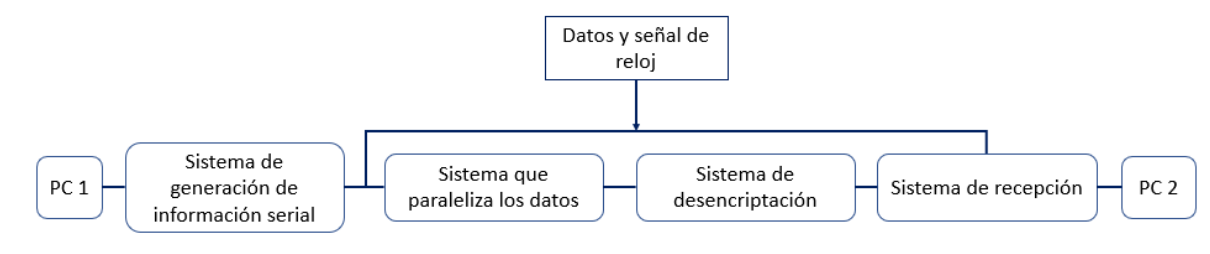
\includegraphics[width=12cm]{imagen/Sistema.png}
    \centering
    \caption{Esquema del sistema  \footnotemark}
    \label{fig:Sistema}
    \end{figure}
   
\footnotetext{Guia del parcial dado por el Profesor Augusto}




\section{75HC595}
\subsection{Un breve vistazo}
El 75HC595 es un circuito integrado digital, recibe los datos de entrada en forma serial,  hasta ocho bits, y entrega sus datos a la salida de forma paralela. 

El circuito integrado 75HC595 tiene un empaquetado de 16 puertos, donde el norte se caracteriza por una entrada de medio óvalo. Los datos los recibe por el pin SER  y la salida de datos en paralelo se da por los pines Qa al Qh. Se tiene también un pin de tierra GND, un pin de energía VCC, un pin Qh' utilizado generalmente para cuando se desean conectar varios de estos integrados en cascadas donde el Qh' salida de un integrado sería la entrada de otro integrado. También se encuentran los pines SRCLK (reloj de registro de desplazamiento) y RCLK (reloj de registro de almacenamiento) correspondientes a la primer y segunda etapa respectivamente. Por último están los pines $\overline{SRCLR}$ y $\overline{OE}$, donde $\overline{OE}$ es el encargado de habilitar o desabilitar los pines de salida mientras que $\overline{SRCLR}$ puede borrar o no los datos del circuito integrado, dependiendo de si su estado es \textit{LOW} o \textit{HIGH}. En la figura \ref{fig:Pines ci} puede obtener una visualización de como están distribuidos los pines.

    \begin{figure}[H]
    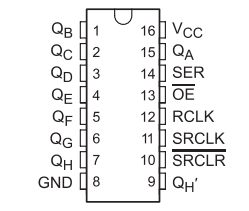
\includegraphics[width=6cm]{imagen/Pines ci.png}
    \centering
    \caption{Vista superior 75HC595\footnotemark}
    \label{fig:Pines ci}
    \end{figure}

\footnotetext{https://www.ti.com/product/SN74HC595}



\newpage
\subsection{Explicación de la esctructura Interna}

En la figura \ref{fig:Estructura Interna} se puede ver la esctructura interna del 75HC595, esta estructura es del proveedor Texas Instruments \cite{Datasheet}, internamente se divide en dos etapas, la etapa uno se encarga del desplazamiento del bit que entra, dicho bit se desplaza por los flipflop, ellos se encuentran conectados en cascada para el desplazamiento del bit, a medida que se va desplazando los bits de entrada la segunda estapa se encarga de almacenarlos, la salida sólo se dará cuando el pin 13 $\overline{OE}$ deje de estar en alta impedancia




\begin{figure}[H]
    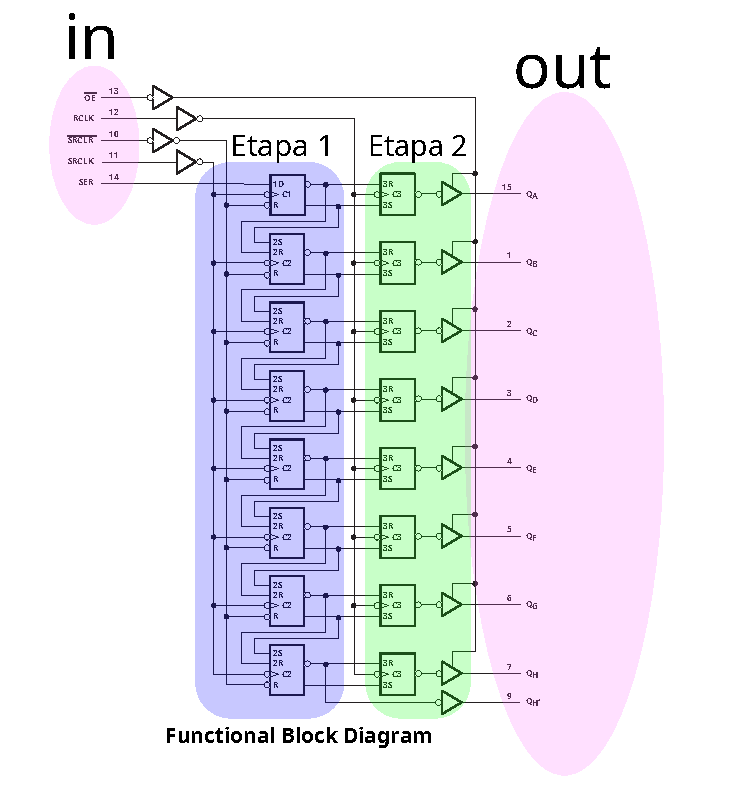
\includegraphics[width=8cm,angle=0, height=10cm ]{imagen/estructuraInterna.pdf}
    \centering
    \caption{Estructura Interna \footnotemark}
    \label{fig:Estructura Interna}
    \end{figure}
    
    \footnotetext{https://www.ti.com/product/SN74HC595}

\subsection{Como conectar el 75HC595}

En la hoja de datos del circuito integrado se encuentra toda la información referente a la forma de realizar las conexiones de los pines.
Los pines Qa al Qh son los pines de salida donde se obtendran los datos de forma paralela. El pin GND se conecta a la tierra del sistema. El pin VCC es la energía del dispositivo, para este proyecto en particular se conecta al puerto que entrega 5v de la placa arduino. Al pin SER se conectan los datos de entrada, los cuales ingresan en forma serial. En cuanto a los pines RCKL y SRCLK, los cuales como ya se mencionó anteriormente, son los relojes del circuito integrado, para este proyecto se conectan cada uno a un pin de salida de la placa arduino por donde haremos envío de la señal de reloj. Por su parte el pin $\overline{OE}$ se conecta a tierra para que quede en estado \textit{LOW}, pues estando en \textit{LOW} activa las salidas lo cual es precisamente lo que necesitamos. El pin $\overline{SRCLR}$ se conecta a VCC para desactivarlo, pues de tenerlo activado borraría el registro. 
La conexión descrita se deduce con ayuda del cuadro \ref{fig:Modos}.


    \begin{figure}[H]
    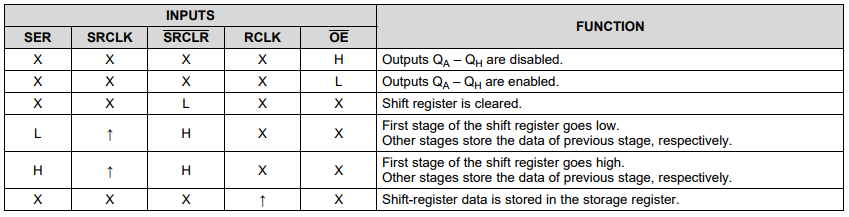
\includegraphics[width=12cm]{imagen/Modos.png}
    \centering
    \caption{Modos funcionales 75HC595\footnotemark}
    \label{fig:Modos}
    \end{figure}
    
    \footnotetext{https://www.ti.com/product/SN74HC595}

    
    
\subsection{Aplicaciones y algunos ejemplos}
Entre sus aplicaciones se encuentran usos para switches de red, servidores, desplegar información por diodos emisores de luz led, entre otros.

\subsubsection{Ejemplo usando pulsadores}
El equipo DeveloperTeam implementó un ejemplo de uso del 75HC595 en la plataforma Tinkercard, en este ejemplo se utilizan pulsadores para enviar los datos al integrado y para las dos señales de reloj del integrado.



\begin{figure}[H]
    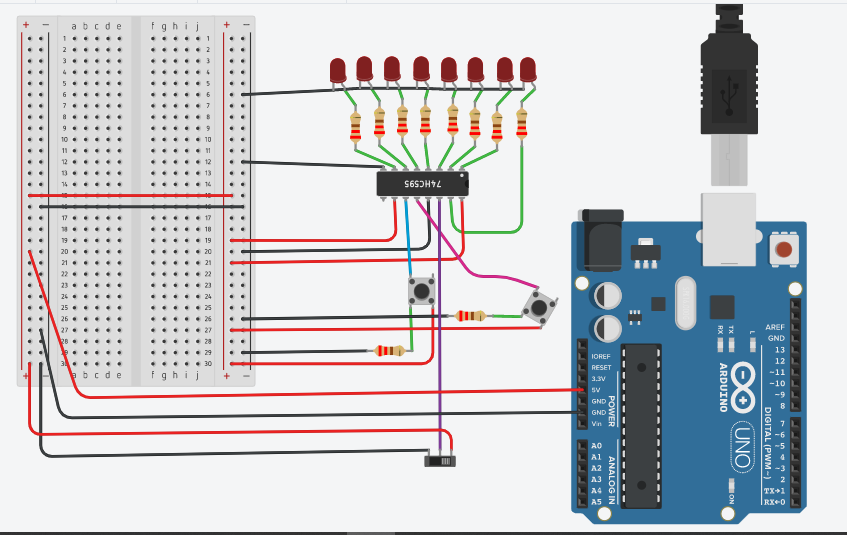
\includegraphics[width=8cm ]{imagen/ej_pulsadores.png}
    \centering
    \caption{Ejemplo uso 74HC595 con pulsadores\footnotemark}
    \label{fig:ej_pulsadores}
    \end{figure}

\footnotetext{https://www.tinkercad.com/things/dO7iXOHbnkA}

\subsubsection{Integrado 74HC595 controlado por Arduino}

\begin{figure}[H]
    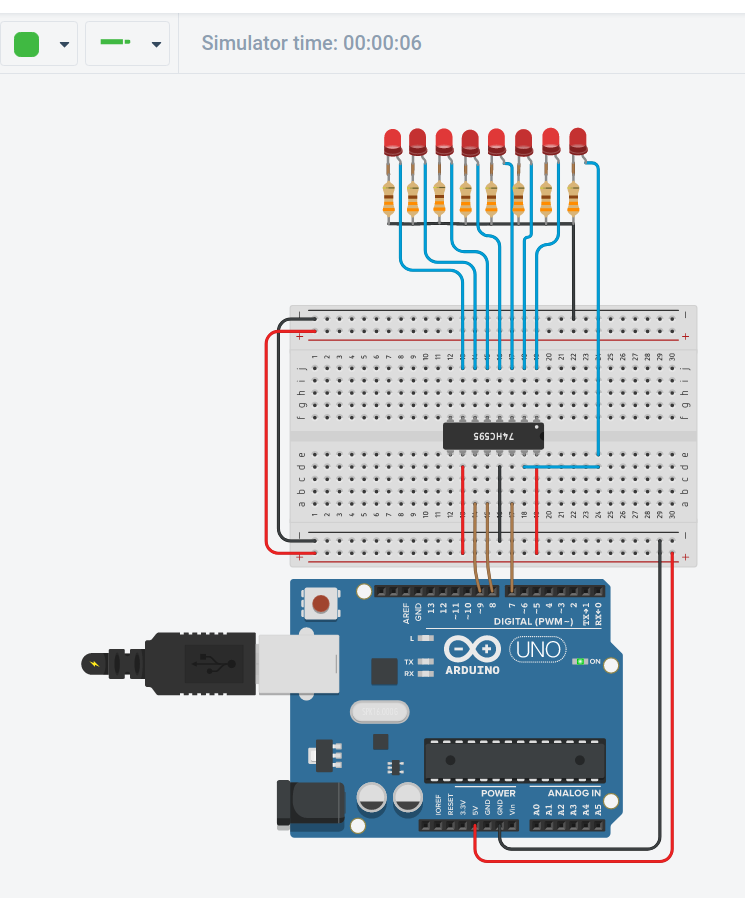
\includegraphics[width=8cm,angle=0, height=10cm]{imagen/74HC595_Arduino.png}
    \centering
    \caption{74HC595 con código en Arduino\footnotemark}
    \label{fig:74HC595_Arduino}
    \end{figure}

\footnotetext{https://www.tinkercad.com/things/86uq2ecFPkF}



\begin{lstlisting}[language=c,commentstyle=\color{miverde},basicstyle=\ttfamily,caption= Código C++,frame=single,]


#define SER 7     // pin 7 a SER del 74HC595
#define RCLK 8    // pin 8 a RCLK del 74HC595
#define SRCLK 9   // pin 9 a SRCLK del 74HC595


int main()
{

  init();
    
      pinMode(SER, OUTPUT);		// pin establecido como salida
      pinMode(RCLK, OUTPUT);	// pin establecido como salida
      pinMode(SRCLK, OUTPUT);	// pin establecido como salida
      
  
  while(1){
    
      digitalWrite(SER, 1);
      
      digitalWrite(SRCLK, 0);
      digitalWrite(RCLK, 0);
      digitalWrite(SRCLK, 1);
      digitalWrite(RCLK, 1);
      delay(500);
      
      
      digitalWrite(SER, 0);
     
      digitalWrite(SRCLK, 0);
      digitalWrite(RCLK, 0);
      digitalWrite(SRCLK, 1);
      digitalWrite(RCLK, 1);
      delay(500);
  }//Fin while
}//Fin main


\end{lstlisting}

En el ejemplo de la figura \ref{fig:74HC595_Arduino} seguido de su código, se usa para mostrar el corrimiento de una entrada serial de 1,0 indefinidamente hasta que se detenga la simulación




\section{Explicación de la arquitectura} 
\subsection{Encriptación}
El usuario entrega el archivo con la información la cual ya está encriptada. Las reglas de encriptación para el \textit{DeveloperTeam} son desconocidas.

\subsection{Transmisión}

\subsection{Desencriptación}
Para desencriptar la información se deben tener en cuenta las reglas de encriptación las cuales son dadas por el profesor Augusto Salazar.

\subsection{Recepción}


\section{Explicación del código fuente} 
 
\label{Elaboracion}



\section{Conclusiones} 
\label{Algoritmo}

\bibliographystyle{IEEEtran}
\bibliography{references}

\end{document}